\documentclass[serif, aspectratio=169]{beamer}
%\documentclass[serif]{beamer}  % for 4:3 ratio

\usepackage[T1]{fontenc} 
\usepackage[utf8]{inputenc}
\usepackage{fourier} % see "http://faq.ktug.org/wiki/uploads/MathFonts.pdf" for other options
\usepackage{hyperref}
\usepackage{latexsym,amsmath,xcolor,multicol,booktabs,calligra}
\usepackage{graphicx,pstricks,listings,stackengine}
\usepackage{lipsum}
\usepackage{../HKUSTstyle}

%imports customs%
\usepackage{caption}    % for subfigures
\usepackage{subcaption} % for subfigures
\usepackage{ragged2e}
\usepackage{booktabs,makecell}
\usepackage{colortbl}
\usepackage{multirow}
\usepackage{cite}
\usepackage{tcolorbox}
\usepackage[sort,authoryear]{natbib}

\author{Julien Bezançon}

\title{Découverte du Traitement Automatique des Langues}
\subtitle{CM 1~: Bienvenue et introduction}

\institute{julien.bezancon@univ-lorraine.fr / \url{https://julienbez.github.io}}

\date{}

% defs
\def\cmd#1{\texttt{\color{red}\footnotesize $\backslash$#1}}
\def\env#1{\texttt{\color{blue}\footnotesize #1}}

% set colors
\definecolor{hkustyellow}{RGB}{167, 131, 55}
\definecolor{hkustblue}{RGB}{0, 56, 116}
\definecolor{hkustred}{RGB}{209, 51, 59}

% easy colors
\newcommand{\tred}[1]{\textcolor{red!50}{#1}}
\newcommand{\tgreen}[1]{\textcolor{green}{#1}}
\newcommand{\tyellow}[1]{\textcolor{yellow}{#1}}
\newcommand{\tpurple}[1]{\textcolor{purple!50}{#1}}

% CLI environment
\newenvironment{CLI} % Command Line Interface
    {
    \noindent
    \ttfamily 
    \footnotesize
    \begin{tcolorbox}[colback=gray!150,colframe=black]
    \color{white}
    \begin{tabular}{p{4.5cm}p{7.5cm}}
    }
    { 
    \end{tabular}
    \end{tcolorbox}
    }

% Exercice environment
\newenvironment{exoframe}
    {
    \setbeamercolor{background canvas}{bg=hkustblue}
    \renewcommand\thefootnote{\textcolor{white}{\arabic{footnote}}}
    \color{white}
    \setbeamercolor{structure}{fg=white}
    \begin{frame}
    }
    {
    \end{frame}
    }

\lstset{
    basicstyle=\ttfamily\small,
    keywordstyle=\bfseries\color{deepblue},
    emphstyle=\ttfamily\color{deepred},    % Custom highlighting style
    stringstyle=\color{deepgreen},
    numbers=left,
    numberstyle=\small\color{halfgray},
    rulesepcolor=\color{red!20!green!20!blue!20},
    frame=shadowbox,
}

\begin{document} %  --- --- --- --- --- --- --- --- --- --- --- --- 

\begin{frame}[noframenumbering,plain]
    \titlepage
    \vspace*{-0.6cm}
    \begin{figure}[htpb]
        \begin{center}
            \hspace{0.3cm}
            
\includegraphics[width=0.7\columnwidth]{../../../IMAGES/loria_idmc.png}
        \end{center}
    \end{figure}
\end{frame}

% \begin{frame}    
%     \tableofcontents[sectionstyle=show,
%     subsectionstyle=show/shaded/hide,
%     subsubsectionstyle=show/shaded/hide]
% \end{frame}

\section{Avant de commencer...}

\begin{frame}{Moi} %Julien Bezançon

    % \begin{figure}
    %     
\includegraphics[width=0.5\columnwidth]{../../../FIGURES/photos/profile_thug.jpeg}
    % \end{figure}

    \begin{minipage}{0.45\columnwidth}
        \begin{figure}
            
\includegraphics[width=0.7\columnwidth]{../../../FIGURES/photos/profile_thug.jpeg}
        \end{figure}
    \end{minipage}
    \begin{minipage}{0.45\columnwidth}
        \begin{block}{Vous me verrez aussi en...}
            \vspace{5pt}
            \begin{itemize}
                \item Data Storage and Retrieval \hfill M1
                \item Prompt Engineering \hfill M2
                \item Software Projects \hfill M2
                \item Written Corpora \hfill M2
                \item Lexicology \hfill M2
            \end{itemize}
        \end{block}
    \end{minipage}
\end{frame}

\begin{frame}{Ce cours} %-- 8 weeks, 4 hours a week
    \begin{block}{10 cours magistraux sur le Traitement Automatique des Langues (TAL)}
        \begin{itemize}
            \item Le TAL~: c'est quoi ?
            \item Les langues naturelles comme données
            \item Les grandes approches du TAL
            \item Traiter et représenter des données langagières
            \item Le TAL dans notre société
        \end{itemize}
    \end{block}
    \begin{block}{Mode d'évaluation}
        \begin{itemize}
            \item Participation orale (10~\%) 
            \item Examen final (90~\%)
            \item Peut-être un TD évalué...
        \end{itemize}
    \end{block}
    \hfill \textbf{Examen final~: ???}
\end{frame}

\begin{frame}{Les travaux dirigés}
    \begin{block}{Deux intervenantes (pas moi !)}
        \begin{itemize}
            \item Clémentine Bleuze (clementine.bleuze@univ-lorraine.fr)
            \item Iglika Nikolova-Stoupak (iglika.nikolova-stoupak@univ-lorraine.fr)
        \end{itemize}
    \end{block}
\end{frame}

\begin{frame}{Références de ce cours}
    \begin{itemize}
        \item Gaël Lejeune (gael.lejeune@sorbonne-universite.fr)
        \begin{itemize}
            \item cours d'ingénierie des langues
        \end{itemize}
        \vspace{10pt}
        \item Xavier Tannier (xavier.tannier@sorbonne-universite.fr)
        \begin{itemize}
            \item cours d'introduction au TAL\footnote{\url{https://etal2023.lis-lab.fr/programme/}}
        \end{itemize}
        \vspace{10pt}
        \item Karën Fort (karen.fort@univ-lorraine.fr)
        \begin{itemize}
            \item cours et travail sur l'éthique
        \end{itemize}
        \vspace{10pt}
        \item Anne-Laure Ligozat (anne-laure.ligozat@lisn.fr)
        \begin{itemize}
            \item travail sur l'impact environnemental du numérique
        \end{itemize}
    \end{itemize}
\end{frame}

\section{Le TAL, c'est quoi ?}

\begin{frame}{Le TAL, c'est quoi ?}
    \begin{block}{Définition de Wikipédia\footnote{\url{https://fr.wikipedia.org/wiki/Traitement_automatique_des_langues}}}
        \begin{tcolorbox}
            Le traitement automatique des langues (TAL), en anglais \textit{natural language processing} ou \textit{NLP}, est un domaine multidisciplinaire impliquant la linguistique, l'informatique et l'intelligence artificielle, qui vise à créer des outils de traitement des langues naturelles pour diverses applications.
        \end{tcolorbox}
    \end{block}
    \begin{center}
        \Large Le TAL cherche à \textbf{traiter} \only<1>{la} \only<2->{\underline{les}} langue\only<2->{s} naturelle\only<2->{s} \\
        Le TAL est \textbf{multidisciplinaire}
    \end{center}
\end{frame}

\begin{frame}{Un exemple}
    \begin{figure} %TODO : trouver ref
        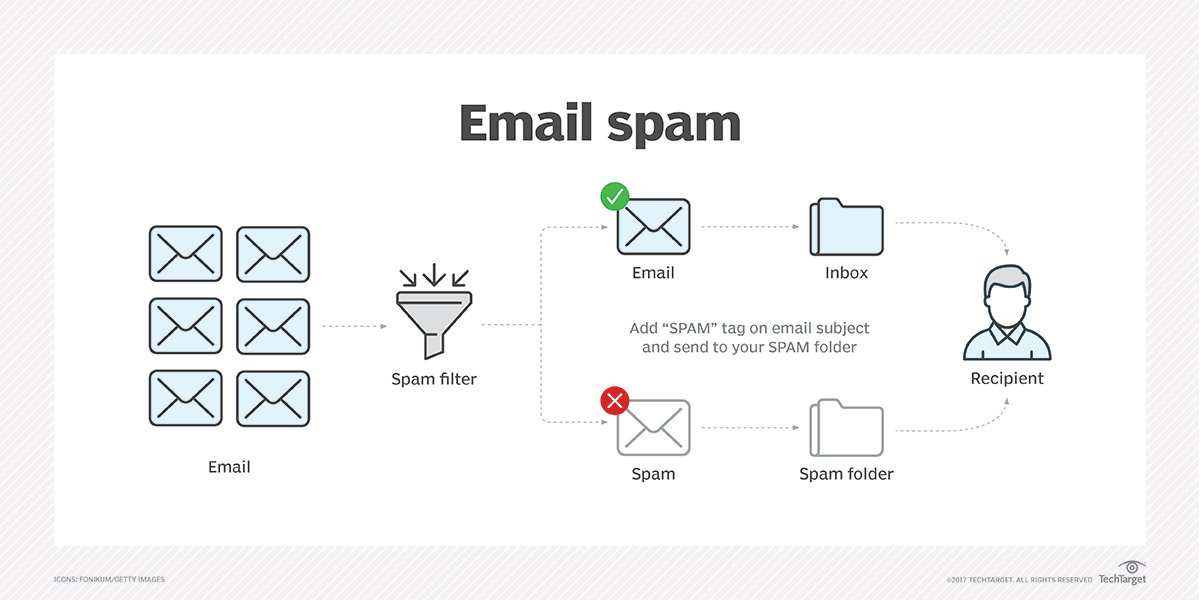
\includegraphics[width=0.8\columnwidth]{../../../FIGURES/découverte_tal/mail_spam_filter.jpg}
        \caption*{Source~: un article d'Andrew Zola\footnote{\url{https://www.techtarget.com/cybersecurity/definition/spam-filter}}}
    \end{figure}
\end{frame}

\begin{frame}{Et le TAL, c'est facile ?}
    \begin{figure} %TODO : trouver ref
        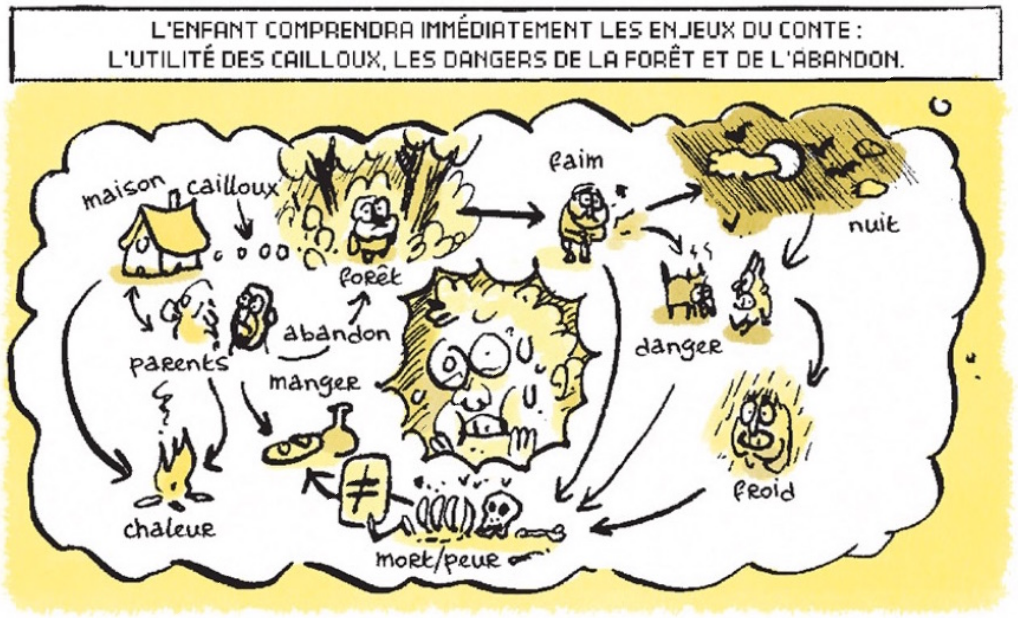
\includegraphics[width=0.8\columnwidth]{../../../FIGURES/découverte_tal/BD_1.png}
    \end{figure}
\end{frame}

\begin{frame}{Et le TAL, c'est facile ?}
    \begin{figure} %TODO : trouver ref
        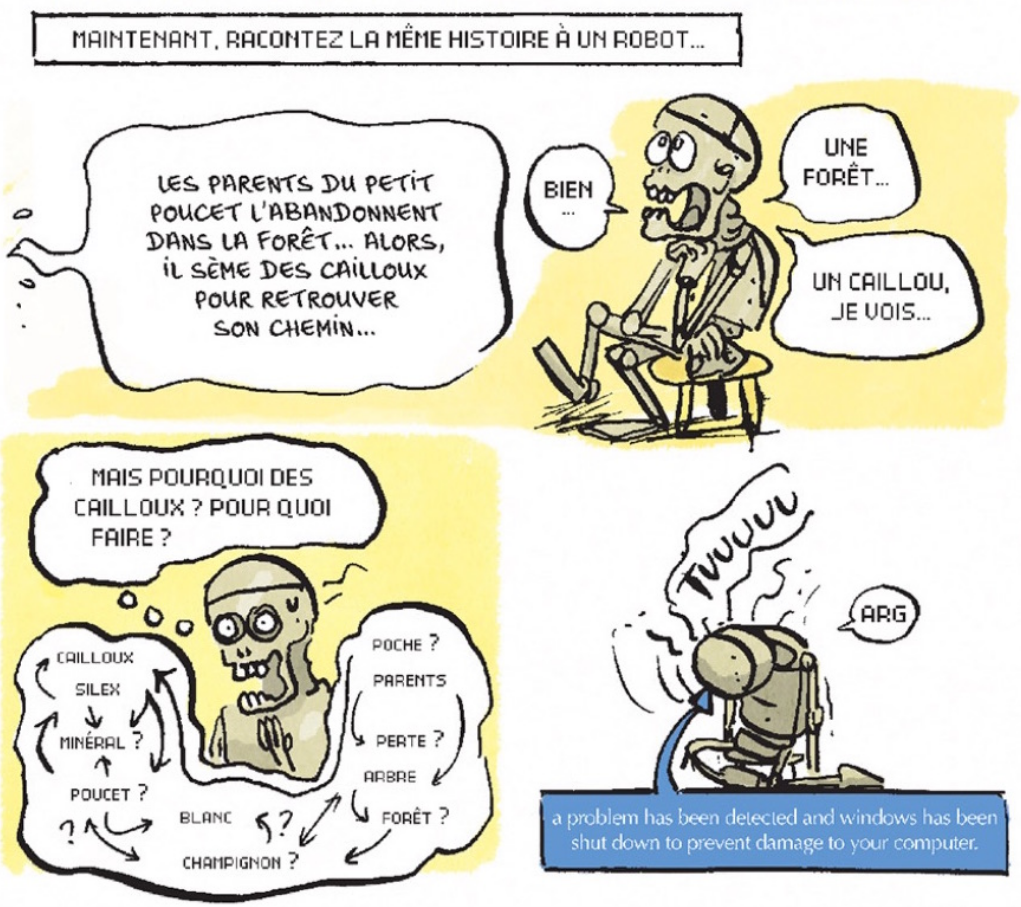
\includegraphics[width=0.55\columnwidth]{../../../FIGURES/découverte_tal/BD_2.png}
    \end{figure}
\end{frame}

% \begin{frame}{Et le TAL, c'est facile ?}
%     \begin{block}{Pourquoi le robot crashe ?}
%         \begin{itemize}
%             \item 
%         \end{itemize}
%     \end{block}
% \end{frame}

\begin{frame}{Problématique}
    \begin{block}{Le langage naturel est...}
        \begin{itemize}
            \item redondant
            \item ambigu
            \item implicite
            \item vivant
            \vspace{15pt}
            \item bref, il est naturel
        \end{itemize}
    \end{block}
    \begin{center}
        \Large Conséquence~: il est difficile à \textbf{représenter}
    \end{center}
\end{frame}

\begin{frame}{Le langage est redondant}
    \begin{figure}
        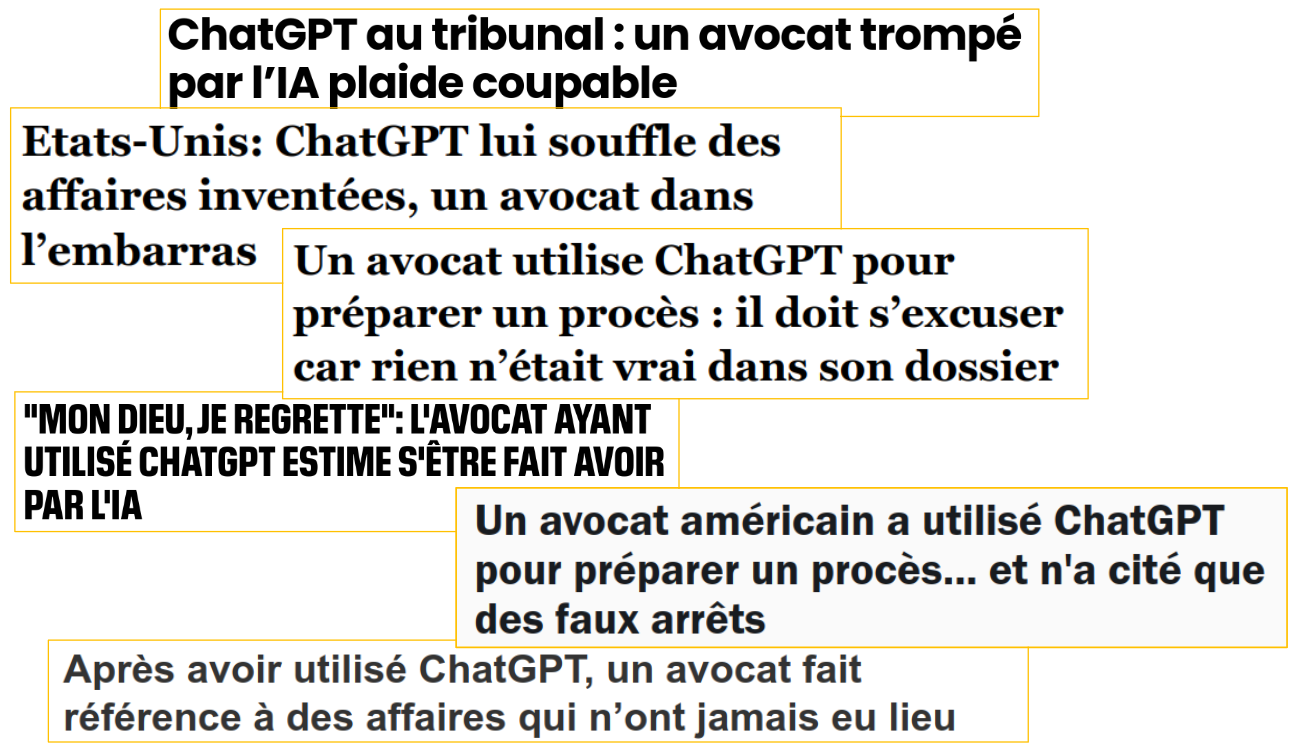
\includegraphics[width=0.8\columnwidth]{../../../FIGURES/découverte_tal/langage_redondant.png}
        \caption*{Source~: Cours d'introduction au TAL de Xavier Tannier}
    \end{figure}
\end{frame}

\begin{frame}{Le langage est ambigu}
    \begin{figure}
        
\includegraphics[width=0.8\columnwidth]{../../../FIGURES/découverte_tal/baguette.png}
    \end{figure}
\end{frame}

\begin{frame}{Le langage est ambigu}
    \begin{block}{}
        \begin{itemize}
            \item L'humain observe le pigon. Il pond un oeuf.
            \begin{itemize}
                \item qui pond un oeuf ? 
                \item $\Rightarrow$ à qui fait référence "il" ?
            \end{itemize}
            \pause
            \vspace{15pt}
            \item Mangez les enfants !
            \begin{itemize}
                \item mieux avec la virgule...
                \item quel sens avez-vous compris en premier ? 
            \end{itemize}
            \pause
            \vspace{15pt}
            \item Il prend des vessies pour des lanternes
            \begin{itemize}
                \item hein ???
                \item les expressions nécéssitent une connaissance préalable
            \end{itemize}
        \end{itemize}
    \end{block}
\end{frame}

\begin{frame}{Le langage est implicite}
    \begin{figure}
        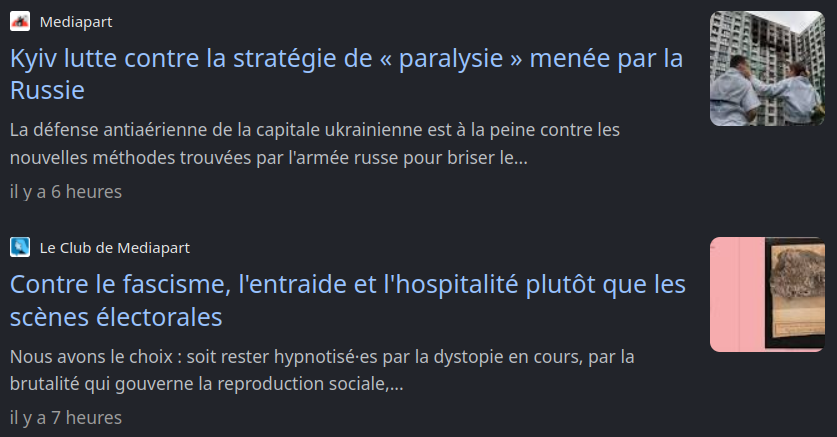
\includegraphics[width=0.8\columnwidth]{../../../FIGURES/découverte_tal/news_implicite.png}
        \caption*{Titre et chapô d'articles de Médiapart (04/09/2026).}
    \end{figure}
\end{frame}

\begin{frame}{Le langage est vivant}
    \begin{minipage}{0.50\columnwidth}
        \begin{figure}
        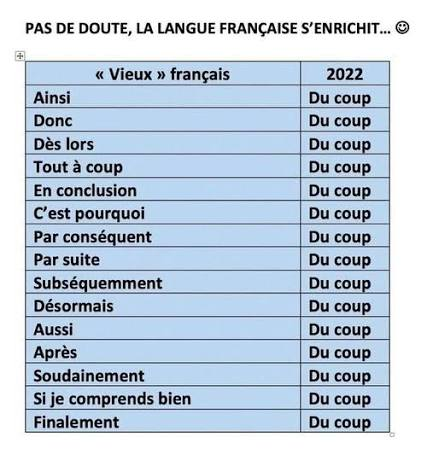
\includegraphics[width=0.8\columnwidth]{../../../FIGURES/découverte_tal/meme_langue_evolution.jpeg}
        \caption*{Un meme (source anonyme).}
    \end{figure}
    \end{minipage}
    \pause
    \begin{minipage}{0.40\columnwidth}
        \vspace{-15pt}
        \begin{block}{Écriture inclusive, néologie, etc}
            \begin{itemize}
                \item aplaventrisme
                \item prompt
                \item dinguerie
                \item quoicoubeh
                \item ...
                \vspace{15pt}
                \item Et vos néologismes ?
            \end{itemize}
        \end{block}
    \end{minipage}
\end{frame}

\begin{frame}{Le langage selon une machine}
    \begin{block}{Ce que "voit" une machine}
        \begin{table}
            \renewcommand{\arraystretch}{1.5}  
            \raggedright
            \begin{tabular}{|l|l|}
                \hline
                Séquence (caractères) & Êl síla erin lû e-govaned vîn \\
                \hline
            \end{tabular}
        \end{table}   
    \end{block}
    \pause
    \begin{block}{Ce qu'elle ne voit et/ou ne comprend pas}
        \begin{table}
            \renewcommand{\arraystretch}{1.5}  
            \raggedright
            \begin{tabular}{|l|l|}
                \hline
                Syntaxe (structure) & \fcolorbox{black}{red!20}{\fcolorbox{black}{red!20}{Êl} \fcolorbox{black}{red!20}{síla} \fcolorbox{black}{red!20}{erin}} \fcolorbox{black}{blue!20}{\fcolorbox{black}{blue!20}{lû} \fcolorbox{black}{blue!20}{e-govaned} \fcolorbox{black}{blue!20}{vîn}} \\
                \hline
                Signifié (sens) & Une étoile brille sur l'heure de notre rencontre \\
                \hline
                Prosodie (oralité) & \textit{$\varepsilon$:l si.la $\varepsilon$.rin lu: $\varepsilon$ go.va.n$\varepsilon$d vi:n} \\
                \hline
                Contexte & \textit{Vous êtes un hobbit saluant gracieusement un elfe} \\
                \hline
            \end{tabular}
        \end{table}
    \end{block}
\end{frame}

\begin{frame}
    \begin{center}
        \Large
        Une machine ne comprend pas le langage. \\
        Une machine ne dispose pas de connaissances de notre monde.
        
        \pause
        \vspace{15pt}
        On peut donner des données et des règles à une machine pour reproduire  des processus cognitifs et linguistiques.
    \end{center}
\end{frame}

\begin{frame}{Autres difficultés}
    \begin{block}{Les langues sont nombreuses}
        \begin{itemize}
            \item Combien de langues connaissez-vous ?
            \item Combien de langues dans le monde ? %environs 7000
            \item Combien de langues en France ? %80 officielles, plusieurs centaines en réalité
        \end{itemize}
    \end{block}
    \begin{block}{Les langues sont multimodales}
       \begin{itemize}
            \item Écriture (registre, alphabet, etc)
            \item Parole (ton, prosodie, rythme, etc)
            \item Gestes (langues des signes, gestes symboliques, etc)
            \item ...
        \end{itemize} 
    \end{block}
\end{frame}

\begin{frame}{Les objectifs du TAL}
    \begin{block}{Le TAL, ce n'est pas...}
        \begin{itemize}
            \item comprendre du langage
            \item \textit{prompter} des modèles de langue
        \end{itemize}
    \end{block}
    \begin{block}{Le TAL, ça sert à...}
        \begin{itemize}
            \item Traiter des données en langage naturel (principalement écrit et oral)
            \item Accomplir des tâches en lien avec le langage
            \item Étudier le fonctionnement du langage
        \end{itemize}
    \end{block}
    \begin{center}
        \Large
        Dans un prochain cours~: les applications du TAL
    \end{center}
\end{frame}

\begin{exoframe}{}
    \begin{center}
        \Large
        Mais avant... avez-vous remarqué ? \\
        \pause
        Langue VS Langage \\
        \pause
        \vspace{15pt}
        Langage~: capacité à communiquer \\
        Langue~: outil pour communiquer \\
        \pause
        \vspace{15pt}
        Écriture et parole~: applications de cet outil
    \end{center}
\end{exoframe}

\section{Comment faire du TAL ?}

\begin{frame}{Langages naturels et non naturels}
    \begin{block}{Pour résumer...}
        \begin{itemize}
            \item Humain~: langage naturel
            \item Machine~: langage non naturel
        \end{itemize}
    \end{block}
    \begin{block}{Un exemple de langage non naturel}
        \vspace{2pt}
        \begin{CLI}
            sentence = "Hello World" & \\
            show\_sentence = True & \\
            & \\
            \tyellow{if} show\_sentence \tyellow{is} True: & \\
            ~~\tpurple{print}(sentence) & \\
        \end{CLI}
    \end{block}
    \begin{center}
        \Large
        Autres exemples~: mathématiques, programmes logiques, etc
    \end{center}
\end{frame}

\begin{exoframe}{Exercice~: le filtre à spams}
    \begin{figure} %TODO : trouver ref
        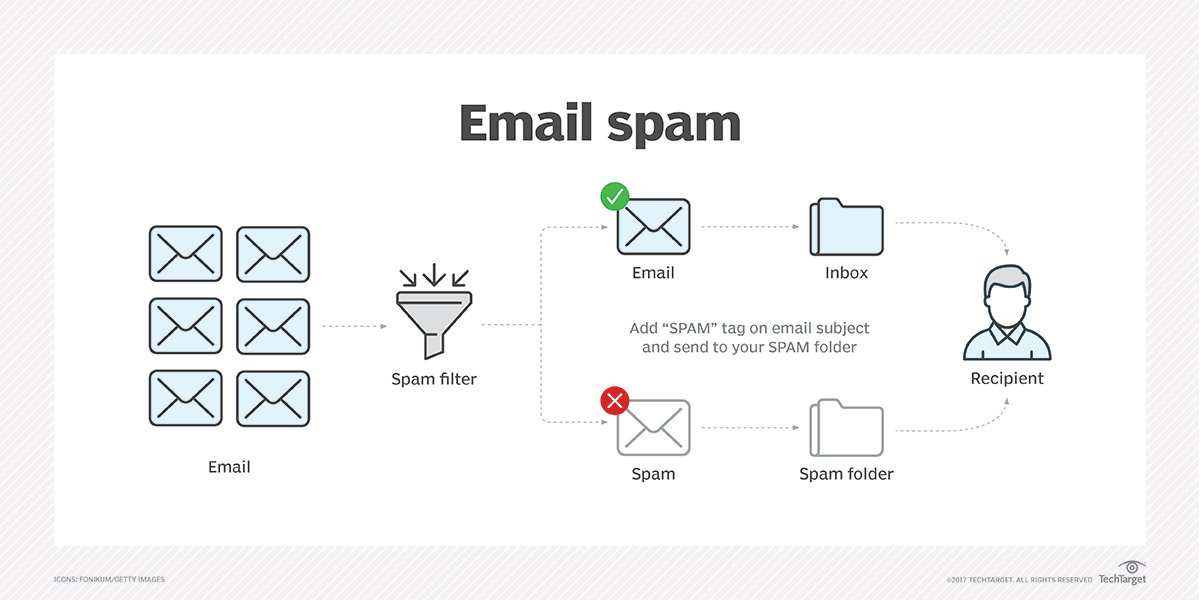
\includegraphics[width=0.8\columnwidth]{../../../FIGURES/découverte_tal/mail_spam_filter.jpg}
        \caption*{\color{white} Source~: un article d'Andrew Zola\footnote{\color{white} \url{https://www.techtarget.com/cybersecurity/definition/spam-filter}}}
    \end{figure}
\end{exoframe}

\begin{exoframe}{Exercice~: le filtre à spams}
    \begin{block}{Un mail est un spam si...}
        \begin{itemize} \color{white}
            \item il contient le mot "urgent"
            \only<1>{\item un riche héritier a besoin d'argent} % contexte improbable, il faut que la machine le repère => transition avec la slide suivante
            \only<2->{\item \underline{un riche héritier a besoin d'argent}}
            \item le domaine mail de l'envoyeur est inconnu
            \item il est envoyé 50 fois en 2 heures
            \item etc
        \end{itemize}
    \end{block}
    \begin{center}
        \Large
        Prochaine étape~: convertir ces observations en consignes \\ pour la machine (= les convertir en langage non naturel)
    \end{center}
\end{exoframe}

\begin{frame}{Le TAL \textbf{EST} multidisciplinaire}
    %expliquer qu'on a besoin de modèles linguistiques pour mieux comprendre comment fonctionne le langage et potentiellement pour les appliquer en informatique
    \begin{block}{Un riche héritier a besoin d'argent}
        \begin{itemize}
            \item Une machine ne comprend pas le langage
            \item Une machine ne dispose pas de connaissances de notre monde
            \item $\Rightarrow$ Analyse du message = complexe
        \end{itemize}
    \end{block}
    \begin{block}{Approches envisagées pour contourner ces problématiques}
        \begin{itemize}
            \item Approches à base de règles (linguistique)
            \item Approches statistiques (mathématiques)
            \item Approches neuronales (neurologie)
        \end{itemize}
    \end{block}
    \begin{center}
        \Large
        Si on comprend un langage, on pourrait le définir \\ pour qu'une machine le comprenne (?)
    \end{center}
\end{frame}

\end{document}
